%%%%%%%%%%%%%%%%%%%%%%%%%%%%%%%%%%%%%%%%%%%%%%%%%%%%%%%%%%%%%%%%%%%%%%
% LaTeX Template: Designer's CV
%
% Source: http://www.howtotex.com
% 
% Feel free to distribute this example, but please keep the referral
% to HowToTeX.com
% 
% Date: March 2012
%
% Modified by Lim Lian Tze to support multiple pages using fix provided at
% http://www.howtotex.com/templates/creating-a-designers-cv-in-latex/
% Date: November 2014
%%%%%%%%%%%%%%%%%%%%%%%%%%%%%%%%%%%%%%%%%%%%%%%%%%%%%%%%%%%%%%%%%%%%%%
% How to use writeLaTeX: 
%
% You edit the source code here on the left, and the preview on the
% right shows you the result within a few seconds.
%
% Bookmark this page and share the URL with your co-authors. They can
% edit at the same time!
%
% You can upload figures, bibliographies, custom classes and
% styles using the files menu.
%
% If you're new to LaTeX, the wikibook is a great place to start:
% http://en.wikibooks.org/wiki/LaTeX
%
%%%%%%%%%%%%%%%%%%%%%%%%%%%%%%%%%%%%%%%%%%%%%%%%%%%%%%%%%%%%%%%%%%%%%%

%%%%%%%%%%%%%%%%%%%%%%%%%%%%%%%%%%%%%
% Document properties and packages
%%%%%%%%%%%%%%%%%%%%%%%%%%%%%%%%%%%%%
\documentclass[a4paper,12pt,final]{memoir}

% misc
\renewcommand{\familydefault}{bch}	% font
\pagestyle{empty}					% no pagenumbering
\setlength{\parindent}{0pt}			% no paragraph indentation


% required packages (add your own)
\usepackage{flowfram}										% column layout
\usepackage[top=1cm,left=1cm,right=1cm,bottom=1cm]{geometry}% margins
\usepackage{graphicx}										% figures
\usepackage{url}											% URLs
\usepackage[usenames,dvipsnames]{xcolor}					% color
\usepackage{multicol}										% columns env.
	\setlength{\multicolsep}{0pt}
\usepackage{paralist}										% compact lists
\usepackage{tikz}

%%%%%%%%%%%%%%%%%%%%%%%%%%%%%%%%%%%%%
% Create column layout
%%%%%%%%%%%%%%%%%%%%%%%%%%%%%%%%%%%%%
% define length commands
\setlength{\vcolumnsep}{\baselineskip}
\setlength{\columnsep}{\vcolumnsep}

% left frame
\newflowframe{0.3\textwidth}{\textheight}{0pt}{0pt}[left]
	\newlength{\LeftMainSep}
	\setlength{\LeftMainSep}{0.22\textwidth}
	\addtolength{\LeftMainSep}{1\columnsep}
 
% small static frame for the vertical line
\newstaticframe{1.5pt}{\textheight}{\LeftMainSep}{0pt}
 
% content of the static frame
\begin{staticcontents}{1}
\hfill
\tikz{%
	\draw[loosely dotted,color=RoyalBlue,line width=1.5pt,yshift=0]
	(0,0) -- (0,\textheight);}%
\hfill\mbox{}
\end{staticcontents}
 
% right frame
\addtolength{\LeftMainSep}{1.5pt}
\addtolength{\LeftMainSep}{1\columnsep}
\newflowframe{0.7\textwidth}{\textheight}{\LeftMainSep}{0pt}[main01]


%%%%%%%%%%%%%%%%%%%%%%%%%%%%%%%%%%%%%
% define macros (for convenience)
%%%%%%%%%%%%%%%%%%%%%%%%%%%%%%%%%%%%%
\newcommand{\Sep}{\vspace{1.5em}}
\newcommand{\SmallSep}{\vspace{0.5em}}

\newenvironment{AboutMe}
	{\ignorespaces\textbf{\color{RoyalBlue} About me}}
	{\Sep\ignorespacesafterend}
	
\newcommand{\CVSection}[1]
	{\Large\textbf{#1}\par
	\SmallSep\normalsize\normalfont}

\newcommand{\CVItem}[1]
	{\textbf{\color{RoyalBlue} #1}}


%%%%%%%%%%%%%%%%%%%%%%%%%%%%%%%%%%%%%
% Begin document
%%%%%%%%%%%%%%%%%%%%%%%%%%%%%%%%%%%%%
\begin{document}

% Left frame
%%%%%%%%%%%%%%%%%%%%
%
% Upload your own photo using the files menu
\begin{figure}
	%\hfill
	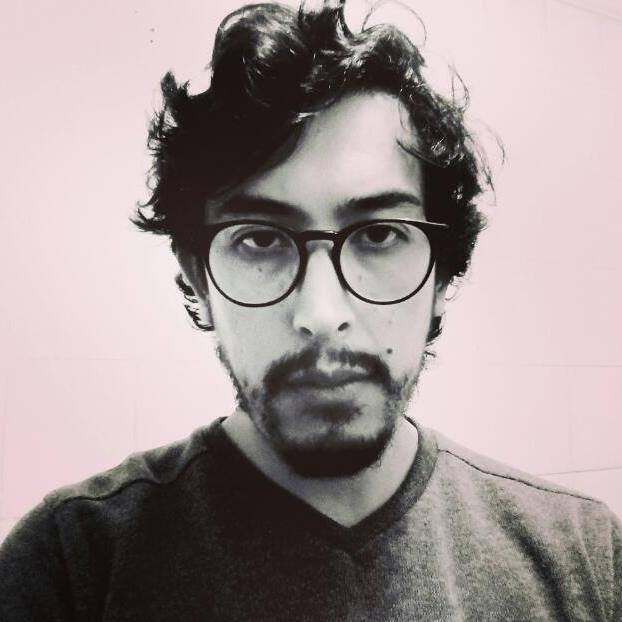
\includegraphics[width=0.75\columnwidth]{my-pic.jpg}
	\vspace{-2cm}
\end{figure}

\begin{flushleft}\small
    \vspace{10mm}
    \textbf{Contact Details}\\
    \vspace{1mm}
	Pablo Ibieta\\
	\vspace{1mm}
	CPF 236.705.918-40 \\
	\vspace{1mm}
    
\includegraphics[width=0.07\columnwidth]{gmail_icon.png} ibieta.pablo@gmail.com \\
    \vspace{1mm}
    
\includegraphics[width=0.08\columnwidth]{usp_icon.png} pibieta@if.usp.br \\
    
\includegraphics[width=0.07\columnwidth]{cellphone_icon.png} (+55) 11 959 410 565 \\	
	\vspace{4mm}
	\textbf{Work Address}\\
	\vspace{1mm}
	Rua do Mat\~ao Travessa R\\
	\vspace{1mm}
	Nr. 187, Off. 331 \\
	\vspace{1mm}
	CEP 05508-090\\
	\vspace{1mm}
	S\~{a}o Paulo, Brazil.\\
	\vspace{4mm}
	\textbf{Personal Address}\\
	\vspace{1mm}
	Rua Frei In\'{a}cio \\
	\vspace{1mm}
	da Concei\c{c}\~{a}o 237, Apto 6 \\
	\vspace{1mm}
	CEP 05362-040 \\
	\vspace{1mm}
	S\~{a}o Paulo, Brazil.\\
	\vspace{4mm}
	\textbf{Details and Publications}\\
	\vspace{1mm}
	Curriculo Lattes \\
	\vspace{1mm}
	https://bit.ly/2CXGU8i\\
	\vspace{1mm}
    
\includegraphics[width=0.07\columnwidth]{in_icon.png} /in/pibieta \\
    \vspace{1mm}
    
\includegraphics[width=0.07\columnwidth]{git.jpeg} /pibieta \\
    \vspace{1mm}
    \vspace{4mm}
	\textbf{Languages}\\
	\vspace{1mm}
	Spanish: Mother tongue\\
	\vspace{1mm}
	English: Fluent\\
	\vspace{1mm}
	Portuguese: Fluent\\
	\vspace{1mm}
	French: Basic
	\vspace{1mm}
\end{flushleft}\normalsize


\framebreak



% Right frame
%%%%%%%%%%%%%%%%%%%%
\Huge\bfseries {\color{RoyalBlue} Pablo Ibieta} \\
\Large\bfseries Physicist \\

\normalsize\normalfont

% About me
\begin{AboutMe}
Since 2012, I have worked as a scientific researcher in the area of Quantum Physics. During this period, I have acquired advanced mathematical knowledge and learned several computational skills concerning data analysis. This involves the manipulation and interpretation of data and the use of statistical tools to compare data to models. In order to complement these skills, currently I am focused on the study and development of Python based Data Science and Machine Learning tools.  
\end{AboutMe}

\vspace{-20pt} 
% Experience
\CVSection{Experience}
\CVItem{Sep 2012 - present}\\
\begin{small}
Junior Researcher and Teaching Assistant,  Instituto de F\'{i}sica, Universidade de S\~{a}o Paulo 
(USP). S\~{a}o Paulo, Brazil. 
Research projects include: 
\end{small}
\begin{footnotesize}
\begin{itemize}
\item Topological phases of matter, quantum physics and mathematical physics.
\item Computer vision for astrophysical image classification.
\item NLP and Deep Learning for ChatBots, both retrieval and generative.
\end{itemize}
\end{footnotesize}

\SmallSep

\CVItem{Oct 2018 - present}\\
{\small Kaggle Competitions participant: \emph{New York City Taxi Fare Predictions} and \emph{Predict Future Sales}}
\SmallSep


\CVItem{Jan 2018}\\
{\small Visiting Professor, Universidad Mayor de San Andr\'{e}s, Physics Department. La Paz, Bolivia.}
\SmallSep

\CVItem{Sep 2005 - Feb 2010}\\
\begin{small}
Junior Researcher and Teaching Assistant. Institute for Theoretical Physics,
UMSA, Physics Department. La Paz, Bolivia. 
\end{small}
%\SmallSep

\SmallSep

% Education
\CVSection{Education}
\CVItem{2015 - 2019}\\
\begin{small}
 Ph. D. in Physics, Universidade de S\~{a}o Paulo (USP).\\ 
S\~{a}o Paulo, Brazil.
 \end{small} 
\SmallSep

\CVItem{2012 - 2015}\\
\begin{small}
M. Sc. in Physics, Universidade de S\~{a}o Paulo (USP)\\
S\~{a}o Paulo, Brazil.
\end{small}
\SmallSep

\CVItem{2004 - 2010}\\
\begin{small}
Bachelor in Physics, Universidad Mayor de San Andr\'{e}s (UMSA).\\
La Paz, Bolivia.
\end{small}

\SmallSep

\CVSection{Skills}

% Skills

\CVItem{Technical}\\
{\small Machine Learning, Neural Networks, Simulations, Feature Engineering, Data Analysis, Visualization, Web.\\}
\vspace{-10pt}
\SmallSep

\CVItem{Software Development}\\
\begin{small}
Python, R, C, C\texttt{++}, Mathematica, SQL, NoSQL, HTML, CSS.\\
Numpy, Pandas, seaborn, matplotlib, openCV, nltk, spacy, Flask, Django, Tensorflow, Keras, sklearn and XGBoost.\\
\end{small}


% References

%\CVSection{References}

%References upon request.

%%%%%%%%%%%%%%%%%%%%%%%%%%%%%%%%%%%%%
% End document
%%%%%%%%%%%%%%%%%%%%%%%%%%%%%%%%%%%%%
\end{document}